%%
%% This is file `./samples/longsample.tex',
%% generated with the docstrip utility.
%%
%% The original source files were:
%%
%% apa7.dtx  (with options: `longsample')
%% ----------------------------------------------------------------------
%% 
%% apa7 - A LaTeX class for formatting documents in compliance with the
%% American Psychological Association's Publication Manual, 7th edition
%% 
%% Copyright (C) 2021 by Daniel A. Weiss <daniel.weiss.led at gmail.com>
%% 
%% This work may be distributed and/or modified under the
%% conditions of the LaTeX Project Public License (LPPL), either
%% version 1.3c of this license or (at your option) any later
%% version.  The latest version of this license is in the file:
%% 
%% http://www.latex-project.org/lppl.txt
%% 
%% Users may freely modify these files without permission, as long as the
%% copyright line and this statement are maintained intact.
%% 
%% This work is not endorsed by, affiliated with, or probably even known
%% by, the American Psychological Association.
%% 
%% ----------------------------------------------------------------------
%% 
\documentclass[man]{apa7}

\usepackage{lipsum}

\usepackage[american]{babel}

\usepackage{tikz}
\usetikzlibrary{shapes.geometric, arrows, positioning, calc}
\usepackage{csquotes}
\usepackage[style=apa,backend=biber]{biblatex}
\addbibresource{bibliography.bib}

\title{Gender Differences in the Impact of Gamification Elements on Performance and Anxiety}
\shorttitle{Gender Differences in the Impact of Gamification Elements}

\authorsnames{Robin Gebert, Nadine Koch, Jun.-Prof. Dr. rer. nat. Maria Wirzberger}
\authorsaffiliations{University of Stuttgart}

\leftheader{Gebert}

\abstract{\lipsum[1]}

\keywords{Gamification, Gender}
%%
%%\authornote{
%%   \addORCIDlink{Daniel A. Weiss}{0000-0000-0000-0000}
%%
%%  Correspondence concerning this article should be addressed to Daniel A. Weiss, Department of Educational Psychology, Counseling and
%%  Special Education, A University Somewhere, 123 Main St., Oneonta, NY
%%  13820.  E-mail: daniel.weiss.led@gmail.com}
%%
\begin{document}
\maketitle


%%
The often mandated transition to remote education during the COVID-19 pandemic highlighted the indispensable role of digital learning environments (DLEs) \parencite{garcia-moralesTransformationHigherEducation2021}.
The usage of digital learning resources saw a significant increase during this period; in 2019, 54\% of students utilized such resources, with the figure rising to 70\% in 2020.
In Germany, the percentage of scholars aged ten to fifteen engaging with digital learning materials doubled from 32\% to 64\% within the same timeframe \parencite{pressestelledesstatistischenbundesamtsDigitalesLernenNimmt2020}.

The integration of gamified elements into DLEs is a common practice, aimed at enhancing motivation and enjoyment \parencite{gonzalezGamificationIntelligentTutoring2014, jacksonMotivationPerformanceGamebased2013}.
However, despite the positive impacts, the introduction of some elements can also lead to negative outcomes, including demotivation \parencite{almeidaSystematicMappingNegative2021}.
The concept of gamification has attracted substantial interest within the educational sciences, becoming a prevalent topic \parencite{swachaStateResearchGamification2021}.
In the realm of computer science, the application of gamified elements is well-documented, demonstrating a important presence due to the inherent integration of technology in the field \parencite{dichevGamifyingEducationWhat2017}.

Although there is extensive research on the general application of gamification, the effects related to individual factors, such as gender, are less understood and warrant further investigation \parencite{dehghanzadehUsingGamificationSupport2024, oliveiraTailoredGamificationEducation2023}.


%% !TeX spellcheck = en_US
%The concept of grading can be seen as a form of gamification, as it adds feedback and a competitive element to the learning process.
%But in recent years especially with the advance of computers, gamification has become an increasingly popular topic in education science \parencite{swachaStateResearchGamification2021}.
%Especially in computer science the use of gamified elements is well researched \parencite{dichevGamifyingEducationWhat2017}, which could be related to the already great use of computers in the field.
%But as this field is still relatively new, many topics are still not well researched, especially how individual factors, such as gender, can influence the effects of gamification \parencite{dehghanzadehUsingGamificationSupport2024,oliveiraTailoredGamificationEducation2023}.
%This thesis aims to explore the effects of different gamified elements and their combinations on performance and anxiety in a digital learning environment, especially focusing on the influence of gender on these effects.
%Digital learning environments, or tutoring systems, were hugely affected by the shift of teaching to remote classes during the COVID-19 pandemic.
%In 2019, 54\% of students utilized digital learning materials, which increased to 70\% the following year. Meanwhile, only 32\% of German scholars aged ten to fifteen engaged with digital learning materials, a figure that doubled to 64\% just one year later.
%Gamification and Digital learning environments are often combined \parencite{gonzalezGamificationIntelligentTutoring2014} with good results \parencite{jacksonMotivationPerformanceGamebased2013} regarding motivation and enjoyment.
%Implementing gamified elements into tutoring systems, while showing positive impact overall, could also lead to negative outcome, for example demotivation while being part of a leaderboard \parencite{almeidaSystematicMappingNegative2021}.
%\textcite{almeidaSystematicMappingNegative2021} also found in their systematic mapping, 77 papers mentioned negative effects like cheating, lack of understanding and most often lack of effect.
%This leads to the question on how gamified digital learning environments could be further improved.
%
%Multiple meta analyses came to the conclusion, further investigation on the effects of different gamification elements on individuals is needed \textcite{oliveiraTailoredGamificationEducation2023,dehghanzadehUsingGamificationSupport2024,hamariDoesGamificationWork2014}, as future systems could also use more individualized data to further enhance the experience of the gamified elements inside the tutoring system.
%Factors mentioned by \textcite{dehghanzadehUsingGamificationSupport2024} include gender and age, \textcite{oliveiraTailoredGamificationEducation2023} mentions culture and gender. All studies highlight the importance of the context, in which the learner is exposed to gamified elements.
%
%Gender could be one of the most significant factors, as it is often discussed in aforementioned studies and was already subject to many studies concerning gamification in different groups and systems.
%\textcite{albuquerqueDoesGenderStereotype2017} which serves as foundation for this paper, investigates the influence of stereotype threat in gendered gamified educational scenarios.
%\textcite{dehghanzadehUsingGamificationSupport2024} showed, that gender is the most controlled factor in their reviewed articles, with mixed outcome. Some studies showed no effect of including gender, others significant differences.
%
%It becomes crucial to expand our understanding of how gender influences the effectiveness of various gamified elements in digital environments. This thesis will assess whether these factors can enhance the learning experience without disadvantaging any gender group.
%Thus, the primary goal is to design digital tutoring systems that fully leverage the potential of gamification to benefit all users equally, fostering an inclusive and effective educational environment.
\section{Theoretical Background}

\subsection{Tutorial systems}
Tutorial systems have become increasingly popular in educational settings, offering a wide range of features and flexibility to support students learning processes.
These systems can range from simple instructive texts to simulations and virtual realities, serving as models that simplify aspects of the real world to reduce complexity mostly from interconnection and context of knowledge for both the machine and the user \parencite{psotkaIntelligentTutoringSystems1988}.
Those Environments are in use at higher education institutions and since the COVID-19 pandemic, they have become more important \parencite{elhadbiReviewStudyAdaptive2024} and widely researched, especially in the field of computer science \parencite{zawacki-richterSystematicReviewResearch2019}.

Tutorial systems are often enhanced with some sort of intelligence (ITS). A dynamic adaptation to learner's needs, incorporating usage factors such as performance, but also external factors such as age, culture or gender \parencite{nkambouAdvancesIntelligentTutoring2010, gonzalezGamificationIntelligentTutoring2014}.
The role of Artificial Intelligence in this process could also become more important in the future, as it could have a significant, yet unknown impact on ITS \parencite{zawacki-richterSystematicReviewResearch2019}.

Tutoring Systems are often used in combination with gamified elements, significantly improving the learning experience \parencite{dermevalGaTOOntologicalModel2019}.
\textcite{jacksonMotivationPerformanceGamebased2013} found that the use of gamified elements in tutoring systems significantly improved the motivation and performance of students compared to traditional tutoring systems which lead to boredom and disengagement after long periods of use.

Incorporating gamified elements not only enhances the engagement and motivation within the ITS but also necessitates mechanisms for tracking progress, such as content unlocking \parencite{gonzalezGamificationIntelligentTutoring2014}.
The evolving landscape of ITS research also includes emotional and relational dynamics, linking student emotions and teacher-student relationships to learning efficacy and motivation \parencite{woolfAffectiveTutorsAutomatic2010}.
These insights have led to the development of digital companions, often named pedagogical agents, within ITS that significantly boost the learning potential and self-concept of students, particularly those who are low-achieving.
Intriguingly, a study noted that ITS programs with a male companion were muted twice as often as those with a female companion, highlighting potential gender differences that could be explored to enhance the predictive capabilities of the student model \parencite{woolfAffectiveTutorsAutomatic2010}.

%\subsection{Gender}
Gender, as a concept within social sciences, refers to more than the binary categorization of male and female.
It encompasses a range of identities and experiences that are shaped by a complex interplay of biological, psychological, and social factors.
Gender is not solely determined by biological characteristics; instead, it is increasingly recognized as a spectrum, acknowledging the presence of diverse gender identities beyond the traditional binary understanding \parencite{lindqvistWhatGenderAnyway2021}.
Socialization plays a critical role in shaping gender identity. It influences how individuals perceive themselves and interact with their surroundings based on the gender norms prevalent within their society.
These norms dictate behaviours, roles, and expectations, which are often internalized from an early age through various socialization agents like family, media, educational institutions, and peer groups \parencite{kampshoffHandbuchGeschlechterforschungUnd2012}.
While acknowledging the spectrum of gender identities, this thesis will focus primarily on the binary categorization of gender—male and female.
This approach does not negate the validity of non-binary or genderqueer identities but rather limits the scope of investigation to traditional gender roles within the binary framework.

Gender is a critical variable to consider when deploying tutorial systems due to its significant influence on learning preferences and outcomes.
Research indicates that male and female students exhibit distinct preferences for learning modalities and react differently to adaptive learning technologies.
For instance, studies have shown that while male students often prefer multimodal instructional approaches, female students tend to favor single-mode learning, particularly kinesthetic styles \parencite{wehrweinGenderDifferencesLearning2007}.
Additionally, the use of adaptive learning technologies has demonstrated a more pronounced improvement in performance among male students compared to their female counterparts in subjects like Mathematics and Portuguese \parencite{desantanaEvaluatingImpactMars2016}.
Moreover, technological proficiency and communication challenges in online settings have been identified as factors affecting learning satisfaction, with older students showing a stronger preference for face-to-face learning, which may be due to less familiarity with digital technologies \parencite{dabajRoleGenderAge2009}.
Recognizing and addressing gender differences in learning styles and preferences is essential for tailoring educational technologies and strategies, thereby optimizing tutorial systems to enhance learning efficacy and engagement for all students.

The design of virtual classroom environments significantly influences gender disparities in computer science courses, impacting both course selection and anticipated success.
Research by \textcite{cheryanClassroomsMatterDesign2011} shows that altering the design of virtual classrooms from stereotypical computer science environments  to more neutral or non-stereotypical settings (e.g., featuring art, nature posters) can substantially increase women's interest and perceived success in computer science.
This change in environment reduces the gender gap by fostering a greater sense of belonging among female students, which is not as pronounced in male students.

%\subsection{Gamification}
Gamification can be defined as "the idea of using game design elements in non-game contexts" \parencite{deterdingGameDesignElements2011} to further increase motivation and user activity within interaction design \parencite{deterdingGameDesignElements2011}.
These game-design elements, subsequently called gamified elements, are elements often found in classical video games. However, the concept of gamification is different from designing a game, the focus lies on using the addictive component \parencite{gonzalezGamificationIntelligentTutoring2014}. Often used elements are points, badges, leaderboards, avatars, and narrated content. Other mechanisms include content unlocking, storytelling, and memes \parencite{zainuddinImpactGamificationLearning2020}.
Often those elements are used in specific constellations like the PBL triad described by \textcite{werbachWinHowGame2012}, which contains points, badges, and leaderboards.
A system that is not only known from games, but also everyday enterprise features like loyalty programs and employee competitions \parencite{werbachWinHowGame2012}.

\begin{APAitemize}
    \item Points, because they add an absolute scale, allowing for quantifiable measurement of user achievements \parencite{hamariDoesGamificationWork2014}.
    \item Badges, because they represent a status symbol and work like a temporary goal to strive toward, often reflecting mastery or achievement \parencite{gonzalezGamificationIntelligentTutoring2014}.
    \item Leaderboards, to compare oneself to peers, which can motivate through social comparison but may also demotivate if not designed carefully \parencite{hamariDoesGamificationWork2014, almeidaSystematicMappingNegative2021}.
    \item Avatars, as they allow users to customize their virtual representation, enhancing their identification with the activity and increasing engagement \parencite{gonzalezGamificationIntelligentTutoring2014}.
    \item Narrated content, which uses storytelling to provide context to activities, thus enriching the user's experience by embedding tasks within an appealing story \parencite{gonzalezGamificationIntelligentTutoring2014}.
\end{APAitemize}
Narrated content or storytelling and avatars are particularly interesting as there appears to be comparatively little research available on these elements, unlike the more extensively studied points, badges, and leaderboards, which was observed during the literature review.
One of the positive effects of gamification is brought by the feedback in different forms (task, process, self-regulation, self) either immediate or delayed.
Feedback is one of the most important factors in the relation between education and learning \textcite{sailerGamificationLearningMetaanalysis2020}.
The use of gamified elements showed positive outcomes in multiple studies, in general \parencite{hamariDoesGamificationWork2014} as well as in education specific contexts \parencite{sailerGamificationLearningMetaanalysis2020}.
But gamification, especially some elements like leaderboards, can also lead to negative outcomes. Leaderboards, while motivating through comparison, have been reported to demotivate participants \parencite{almeidaSystematicMappingNegative2021}.
"Pavlovication" as \textcite{klabbersArchitectureGameScience2018} calls it, Gamification, as it is often a short question-answer-reward-cycle, conditions the user to learn conditional and narrows the possible ways to solve a problem down \parencite{klabbersArchitectureGameScience2018}.
Some studies also suggested that gamified learning platforms also lack individualism regarding choice and display of gamification elements, resulting in discomfort and negative emotions \parencite{santosDoesGenderStereotype2023}.
To combat this missing individualism, \textcite{oliveiraTailoredGamificationEducation2023,dehghanzadehUsingGamificationSupport2024} suggest using more independent variables to tailor the use of gamification elements.

%%% !TeX spellcheck = en_US

\section{Foundations and Related Work}
\label{chap:ch2}





You need to differentiate between Foundation and related work. Foundation is a method/concept/discipline.. that you are re-using and to understand your thesis, readers need to know about them. However, related work shows why this problem has not been sufficiently solved before.

\subsection{Foundations}
Here, introduce necessary foundations that is required for understanding your thesis. For example, your research area is on Model-driven software development, and it is necessary for readers to know the concept of model-2-model transformation.
\subsection{Related work}
In addition to discussing about foundations, you need to discuss about why the problem you are tackling has been insufficiently solved before. To do so, you need to mention related work and discuss what is the difference between your work and those related works.
\subsubsection{Literature Research Methodology}
It is important that you write how you collected the literature related to your research. Did you use one or more search engine(s)? What were they? What keyword(s) you used? What were the combination of those keywords?
Hitting search button usually yields many results, what were the quality criteria for including or  excluding a paper from your collection?




LaTeX-Hinweise stehen in %%\cref{chap:latexhints}.

%noch etwas Fülltext
%\blinddocument

\section{Hypotheses}

As noted in the first chapter, there are open questions regarding the efficiency of various gamified elements and how different genders relate to these gamified elements.
To explore the impact of gender and gamification elements regarding performance and anxiety, we have created the following model:\newline

\begin{figure}[H]
    \centering
    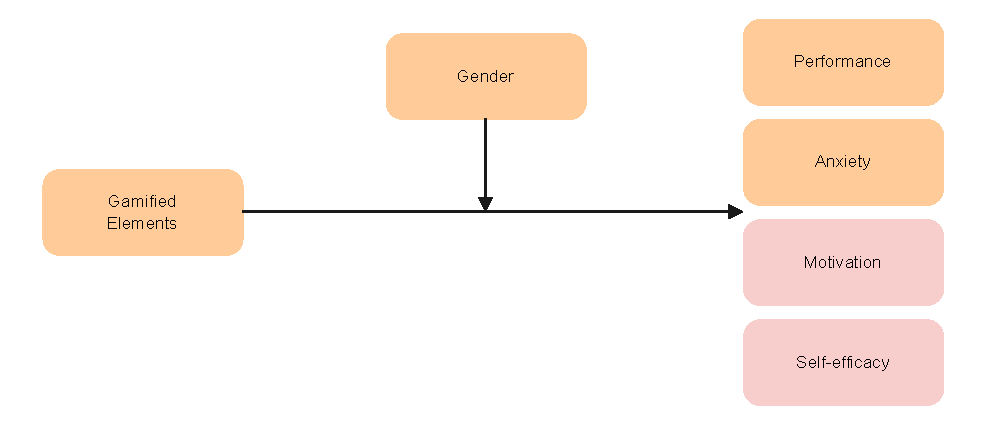
\includegraphics{img/Hypotheses}
    \caption{This diagram illustrates the impact of gamified elements (independent variable) on performance and anxiety (dependent variables), mediated by gender (mediating variable).}
    \label{fig:figureHypotheses}
\end{figure} The hypotheses we want to investigate in this work are:
\begin{itemize}
    \item[H1] Males and females differ in their cognitive and affective states.
    \begin{APAitemize}
        \item[a)] Male performance is better compared to female.
        \item[b)] Male and female students differ regarding their anxiety levels.
    \end{APAitemize}
    \item[H2] Different gamified elements have a varying impact on the cognitive and affective states.
    \begin{APAitemize}
        \item[a)] Gamified elements impact performance differently.
        \item[b)] Different gamified elements impact anxiety levels differently.
    \end{APAitemize}
    \item[H3] Different gamified elements differently impact the cognitive and affective states of males and females.
    \begin{APAitemize}
        \item[a)] The influence of different gamified elements on performance differs between males and females.
        \item[b)] The influence of different gamified elements on anxiety levels differs between males and females.
    \end{APAitemize}
\end{itemize}
%%% !TeX spellcheck = en_US

\section{Chapter three}
\label{chap:ch3}
You design your own chapters, starting from here

%\blinddocument

%%% !TeX spellcheck = en_US

\section{Evaluation}
\label{chap:evaluation}
\subsection{Data Exclusion}
Participants who identified their gender as "other" were excluded from the analysis because the present research available and used for this thesis primarily focuses on comparisons between male and female participants.
This criterion led to the exclusion of two participants. Additionally, participants who achieved less than 25\% correct answers in the gamified learning environment were excluded.
This threshold was set because there were five possible answers for each question, and random clicking would statistically result in a 20\% correct response rate.
Therefore, a performance below 25\% suggests either random guessing or a fundamental misunderstanding of the task.
Furthermore, any incomplete data sets were excluded to ensure the integrity and consistency of the analysis, resulting in the exclusion of one additional participant.
Initially, there were 120 data sets, and after applying the exclusion criteria, 117 data sets remained.

\section{Outline of statistical analysis}
Having preprocessed and cleaned the data, we proceeded with our statistical analysis using linear mixed models (LMMs).
These models were chosen for their ability to handle the complexities of repeated measures from the same subjects under varying conditions.
By incorporating both fixed effects (gender and gamified elements) and random effects (individual differences), LMMs provided a robust framework for our analysis.

We utilized the Nelder-Mead optimization method to estimate the parameters of our models.
This method is ideal for our needs as it efficiently handles models with multiple interacting effects without requiring derivative calculations, making it suitable for our complex dataset.

For the estimation of variance components within our models, we employed Restricted Maximum Likelihood (REML).
REML is preferred in mixed model contexts because it adjusts the estimates for the fixed effects, providing unbiased variance estimates despite the presence of random effects.

Finally, to ensure accurate inference regarding the fixed effects, we applied the Satterthwaite approximation for estimating degrees of freedom.
This method helps in achieving more reliable p-values by adjusting the degrees of freedom for the complexity of the model, crucial in cases with multiple levels of interactions and a limited sample size.

This combination of methods and their implementation through LMMs allowed us to systematically analyse the effects of gender and gamified elements on performance and anxiety, controlling for individual variability and the specifics of the experimental design.

\subsection{Results}

\subsubsection{Performance}
Our analysis revealed no significant main effects or interactions for all hypotheses regarding performance, as documented in Table \ref{tab:lmm_performance}. Despite this lack of significant effects, some descriptive effects are notable.

Women exhibited lower performance levels when leaderboards were the gamified Element used ($M $= .700, $SE$ = .056) compared to men ($M$ = .835, $SE$ = .024) and to the overall average performance in gamified settings for women ($M$ = .846, $SE$ = 0.030). Notable is also the variability suggested by the large standard error for women in this leaderboard condition.

\begin{figure}[h]
    \centering
    \begin{subfigure}[b]{0.45\textwidth}
        \includegraphics[width=\textwidth]{img/plots/plot_performance.png}
        \label{fig:plot_performance}
    \end{subfigure}
    \hfill
    \begin{subfigure}[b]{0.45\textwidth}
        \includegraphics[width=\textwidth]{img/plots/plot_performance_gender.png}
        \label{fig:plot_performance_gender}
    \end{subfigure}
    \caption{On the left: Overall performance across different gamification elements. On the right: Performance differences between genders across different gamified elements.}
    \label{fig:performance_comparison}
\end{figure}

\begin{table}[h]
    \centering
    \caption{Results of the linear mixed model analysis for percentage correct effects.}
    \label{tab:lmm_percentage_correct}
    \resizebox{\textwidth}{!}{
        \begin{tabular}{|l|l|l|l|l|l|}
            \hline
            \textbf{Variable} & \textbf{std. Beta \(\beta\)} & \textbf{standardized 95\% CI of \(\beta\)} & \textbf{\( p \)} & \textbf{Statistic} & \textbf{df} \\
            \hline
            Gender [male] & 0.07 & [-0.47, 0.62] & 0.994 & 0.27 & 277.62 \\
            Gamified Element [Points (P)] & -0.33 & [-0.82, 0.16] & 0.493 & -1.35 & 211.82 \\
            Gamified Element [Badges (B)] & 0.06 & [-0.50, 0.62] & 0.994 & 0.21 & 214.27 \\
            Gamified Element [Level (L)] & -0.48 & [-1.04, 0.09] & 0.384 & -1.67 & 213.69 \\
            Gamified Element [Avatars (A)] & 0.13 & [-0.39, 0.64] & 0.994 & 0.49 & 208.19 \\
            Gamified Element [Narrative Content (N)] & 0.44 & [-0.07, 0.95] & 0.384 & 1.70 & 207.03 \\
            Gamified Element [Combination (PBLA)] & 0.01 & [-0.45, 0.48] & 0.994 & 0.06 & 208.37 \\
            Gamified Element [All Elements (PBLAN)] & 0.06 & [-0.46, 0.57] & 0.994 & 0.22 & 210.22 \\
            Gender [male] × Gamified Element [Points (P)] & 0.42 & [-0.20, 1.04] & 0.493 & 1.33 & 214.33 \\
            Gender [male] × Gamified Element [Badges (B)] & -0.22 & [-0.88, 0.45] & 0.994 & -0.64 & 213.78 \\
            Gender [male] × Gamified Element [Level (L)] & 0.61 & [-0.06, 1.28] & 0.384 & 1.79 & 214.82 \\
            Gender [male] × Gamified Element [Avatars (A)] & 0.01 & [-0.62, 0.64] & 0.994 & 0.03 & 209.52 \\
            Gender [male] × Gamified Element [Narrative Content (N)] & -0.00 & [-0.63, 0.63] & 0.994 & -0.01 & 210.19 \\
            Gender [male] × Gamified Element [Combination (PBLA)] & 0.37 & [-0.25, 0.98] & 0.548 & 1.18 & 211.59 \\
            Gender [male] × Gamified Element [All Elements (PBLAN)] & 0.01 & [-0.63, 0.64] & 0.994 & 0.02 & 210.43 \\
            \hline
        \end{tabular}
    }
\end{table}



\subsubsection{Anxiety}
Similarly, our analysis revealed no significant main effects or interactions for all hypotheses regarding anxiety levels, as detailed in Table \ref{tab:lmm_anxiety}. Nonetheless, some descriptive trends are worth noting.

Figure \ref{fig:plot_anxiety_gender} shows that women experienced higher anxiety levels in the non-gamified environment ($M$ = .571, $SE$ = .092) and with leaderboards ($M$ = .683, $SE$ = .205) compared to men in the same settings ($M$ = .296, $SE$ = .099 and $M$ = .566, $SE$ = .119, respectively). Conversely, the use of avatars led to lower anxiety levels in women ($M$ = .187, $SE$ = .095) compared to men ($M$ = .476, $SE$ = .102 ).

\begin{figure}[h]
    \centering
    \begin{subfigure}[b]{0.45\textwidth}
        \includegraphics[width=\textwidth]{img/plots/plot_anxiety.png}
        \label{fig:plot_anxiety}
    \end{subfigure}
    \hfill
    \begin{subfigure}[b]{0.45\textwidth}
        \includegraphics[width=\textwidth]{img/plots/plot_anxiety_gender.png}
        \label{fig:plot_anxiety_gender}
    \end{subfigure}
    \caption{On the left: Anxiety levels across different gamification elements. On the right: Differences in anxiety levels between genders in various gamification contexts.}
    \label{fig:anxiety_comparison}
\end{figure}

\begin{table}[h]
    \centering
    \caption{Results of the linear mixed model analysis for STAI effects.}
    \label{tab:lmm_stai}
    \resizebox{\textwidth}{!}{
        \begin{tabular}{|l|l|l|l|l|l|}
            \hline
            \textbf{Variable} & \textbf{std. Beta \(\beta\)} & \textbf{standardized 95\% CI of \(\beta\)} & \textbf{\( p \)} & \textbf{Statistic} & \textbf{df} \\
            \hline
            Gender [male] & -0.25 & [-0.83, 0.34] & 0.623 & -0.83 & 288.25 \\
            Gamified Element [Points (P)] & -0.28 & [-0.83, 0.27] & 0.564 & -1.00 & 216.76 \\
            Gamified Element [Badges (B)] & 0.23 & [-0.40, 0.86] & 0.623 & 0.73 & 221.07 \\
            Gamified Element [Leaderboards (L)] & -0.04 & [-0.67, 0.59] & 0.913 & -0.11 & 220.38 \\
            Gamified Element [Avatars (A)] & -0.62 & [-1.20, -0.04] & 0.228 & -2.11 & 213.37 \\
            Gamified Element [Narrative Content (N)] & -0.53 & [-1.10, 0.05] & 0.241 & -1.81 & 211.70 \\
            Gamified Element [Combination (PBLA)] & -0.03 & [-0.55, 0.50] & 0.913 & -0.11 & 213.53 \\
            Gamified Element [All Elements (PBLAN)] & -0.60 & [-1.18, -0.02] & 0.228 & -2.04 & 215.77 \\
            Gender [male] × Gamified Element [Points (P)] & 0.42 & [-0.28, 1.11] & 0.481 & 1.18 & 220.20 \\
            Gender [male] × Gamified Element [Badges (B)] & -0.18 & [-0.93, 0.57] & 0.787 & -0.47 & 220.26 \\
            Gender [male] × Gamified Element [Leaderboards (L)] & 0.28 & [-0.47, 1.04] & 0.623 & 0.74 & 221.54 \\
            Gender [male] × Gamified Element [Avatars (A)] & 0.64 & [-0.07, 1.35] & 0.241 & 1.79 & 214.84 \\
            Gender [male] × Gamified Element [Narrative Content (N)] & 0.50 & [-0.21, 1.21] & 0.437 & 1.40 & 215.47 \\
            Gender [male] × Gamified Element [Combination (PBLA)] & 0.10 & [-0.58, 0.79] & 0.882 & 0.29 & 217.43 \\
            Gender [male] × Gamified Element [All Elements (PBLAN)] & 0.45 & [-0.26, 1.17] & 0.481 & 1.25 & 215.91 \\
            \hline
        \end{tabular}
    }
\end{table}





%\begin{table}[h]
%    \centering
%    \caption{Results of the linear mixed model analysis for performance effects.}
%    \label{tab:lmm_performance}
%    \resizebox{\textwidth}{!}{ % Skaliert die Tabelle auf Textbreite
%        \begin{tabular}{|l|l|l|l|l|l|l|l|l|l|}
%            \hline
%            \thead{Variable} & \thead{Mean\\experimental} & \thead{Mean\\control} & \thead{Estimated\\difference \( d \)} & \thead{\( t \)} & \thead{\( p \)} & \thead{\( df \)} & \thead{95\% LCI\\of \( d \)} & \thead{95\% UCI\\of \( d \)} & \thead{Cohen's \( d \)} \\
%            \hline
%            gender [male] &  &  & .01 & .27 & .994 & 278 & -.06 & .08 & .07 \\
%            gamifiedElement [Points (P)] &  &  & -.04 & -1.35 & .493 & 212 & -.11 & .02 & -.33 \\
%            gamifiedElement [Badges (B)] &  &  & .01 & .21 & .994 & 214 & -.06 & .08 & .06 \\
%            gamifiedElement [Level (L)] &  &  & -.06 & -1.67 & .384 & 214 & -.13 & .01 & -.48 \\
%            gamifiedElement [Avatars (A)] &  &  & .02 & .49 & .994 & 208 & -.05 & .08 & .13 \\
%            gamifiedElement [Narrative Content (N)] &  &  & .06 & 1.70 & .384 & 207 & -.01 & .12 & .44 \\
%            gamifiedElement [Combination (PBLA)] &  &  & .00 & .06 & .994 & 208 & -.06 & .06 & .01 \\
%            gamifiedElement [All Elements (PBLAN)] &  &  & .01 & .22 & .994 & 210 & -.06 & .07 & .06 \\
%            \makecell{gender [male] x \\ gamifiedElement [Points (P)]} &  &  & .05 & 1.33 & .493 & 214 & -.03 & .13 & .42 \\
%            \makecell{gender [male] x \\ gamifiedElement [Badges (B)]} &  &  & -.03 & -.64 & .994 & 214 & -.11 & .06 & -.22 \\
%            \makecell{gender [male] x \\ gamifiedElement [Level (L)]} &  &  & .08 & 1.79 & .384 & 215 & -.01 & .17 & .61 \\
%            \makecell{gender [male] x \\ gamifiedElement [Avatars (A)]} &  &  & .00 & .03 & .994 & 210 & -.08 & .08 & .01 \\
%            \makecell{gender [male] x \\ gamifiedElement [Narrative Content (N)]} &  &  & .00 & -.01 & .994 & 210 & -.08 & .08 & .00 \\
%            \makecell{gender [male] x \\ gamifiedElement [Combination (PBLA)]} &  &  & .05 & 1.18 & .548 & 212 & -.03 & .13 & .37 \\
%            \makecell{gender [male] x \\ gamifiedElement [All Elements (PBLAN)]} &  &  & .00 & .02 & .994 & 210 & -.08 & .08 & .01 \\
%            \hline
%        \end{tabular}
%    }
%\end{table}
%
%Our analysis revealed no significant main effects and no significant interactions for all hypotheses regarding performance and anxiety.
%The results of the linear mixed model analysis for performance effects are shown in Table \ref{tab:lmm_performance}, for anxiety effects in Table \ref{tab:lmm_anxiety}.
%%% !TeX spellcheck = en_US

\section{Conclusion}\label{chap:conclusion}


\subsection{Summary}
... Summarize key aspects and insights, i.e., do not repeat your thesis...
\subsection{Benefits}
... Who (software testers, software developers, software architects,etc.) benefits from your result? In what way?   ..
\subsection{Limitations}
In what settings your approach/method/theory does not hold/work?
\subsection{Lessons Learned}
... What lessons did you learn throughout your thesis that is interesting to be mentioned? For example during experiment setup, or literature review, etc. ... 
\subsection{Future Work}
What is your suggestion for future work?

\end{document}

%% 
%% Copyright (C) 2021 by Daniel A. Weiss <daniel.weiss.led at gmail.com>
%% 
%% This work may be distributed and/or modified under the
%% conditions of the LaTeX Project Public License (LPPL), either
%% version 1.3c of this license or (at your option) any later
%% version.  The latest version of this license is in the file:
%% 
%% http://www.latex-project.org/lppl.txt
%% 
%% Users may freely modify these files without permission, as long as the
%% copyright line and this statement are maintained intact.
%% 
%% This work is not endorsed by, affiliated with, or probably even known
%% by, the American Psychological Association.
%% 
%% 
%% This work is "maintained" (as per LPPL maintenance status) by
%% Daniel A. Weiss.
%% 
%% This work consists of the file  apa7.dtx
%% and the derived files           apa7.ins,
%%                                 apa7.cls,
%%                                 apa7.pdf,
%%                                 README,
%%                                 APA7american.txt,
%%                                 APA7british.txt,
%%                                 APA7dutch.txt,
%%                                 APA7english.txt,
%%                                 APA7french.txt,
%%                                 APA7german.txt,
%%                                 APA7ngerman.txt,
%%                                 APA7greek.txt,
%%                                 APA7czech.txt,
%%                                 APA7turkish.txt,
%%                                 APA7endfloat.cfg,
%%                                 Figure1.pdf,
%%                                 shortsample.tex,
%%                                 longsample.tex, and
%%                                 bibliography.bib.
%% 
%%
%% End of file `./samples/longsample.tex'.
